\documentclass{beamer}
\usepackage{chronosys}
\usepackage{tikz}

\usepackage{ifpdf}
\ifpdf
\usepackage{hyperref}
%\pdfadjustspacing=1
%\fi

\mode<presentation>
 {
  \usetheme{Frankfurt}
   \usecolortheme[rgb={0.36,0.54,0.66}]{structure}
   
   \definecolor{inaf}{HTML}{1D71B8}
   %\definecolor{ashgrey}{rgb}{0.7, 0.75, 0.71}
   \definecolor{autumn}{rgb}{0.7, 0.75, 0.71}
   \definecolor{autumn1}{rgb}{0.7, 0.75, 0.71}
   \definecolor{autumn2}{rgb}{0.36, 0.54, 0.66}
   
   \definecolor{blue}{HTML}{84CECC}
   \definecolor{gr}{HTML}{375D81}

\setbeamercolor{alerted text}{fg=inaf!80!yellow}
\setbeamercolor*{palette primary}{fg=inaf!60!black,bg=autumn}
\setbeamercolor*{palette secondary}{fg=white!70!black,bg=autumn2}
\setbeamercolor*{palette tertiary}{bg=white!80!black,fg=autumn2}
\setbeamercolor*{palette quaternary}{fg=white,bg=autumn2}

\setbeamercolor*{sidebar}{fg=inaf,bg=autumn}

\setbeamercolor*{palette sidebar primary}{fg=inaf!10!black}
\setbeamercolor*{palette sidebar secondary}{fg=white}
\setbeamercolor*{palette sidebar tertiary}{fg=inaf!50!black}
\setbeamercolor*{palette sidebar quaternary}{fg=yellow!10!orange}

\setbeamercolor*{titlelike}{parent=palette primary}
\setbeamercolor{frametitle}{bg=autumn1}
\setbeamercolor{frametitle right}{bg=autumn}

\setbeamercolor*{separation line}{}
\setbeamercolor*{fine separation line}{}

\mode
<all>
   
   %\usecolortheme{wolverine}
   \usecolortheme{rose}
   \usefonttheme{serif}
%   \setbeamercolor{section in toc}{fg=red}
 }

\title[Quantum world]{Il meraviglioso mondo quantistico}
\author[G.Filippelli]{Gianluigi Filippelli}
\date{Liceo "C. Cavalleri", Parabiago (Milano). 09/02/2018}

\usepackage[latin1]{inputenc}
\usepackage[italian]{babel}
\usepackage{times}
%
\begin{document}
%
\begin{frame}
 \titlepage
\end{frame}
%
% La costante di Planck
%
\section{La costante di Planck}
%
\begin{frame}[timeline01]
	\frametitle{Quando inizia il XX secolo della fisica}
	%---------------------timeline----------------%
	\startchronology[align=left, startyear=1897,stopyear=1922, height=0pt, startdate=false, stopdate=false, dateselevation=0pt, arrow=false, box=true]
	%
	\chronograduation[event][dateselevation=0pt]{1}
	%---------------------periods----------------%
	\chronoperiode[textstyle=\raggedleft\colorbox{inaf!50}, color=gr, startdate=false, bottomdepth=0pt, topheight=8pt, textdepth=-25pt,dateselevation=16pt, stopdate=false]{1899}{1900}{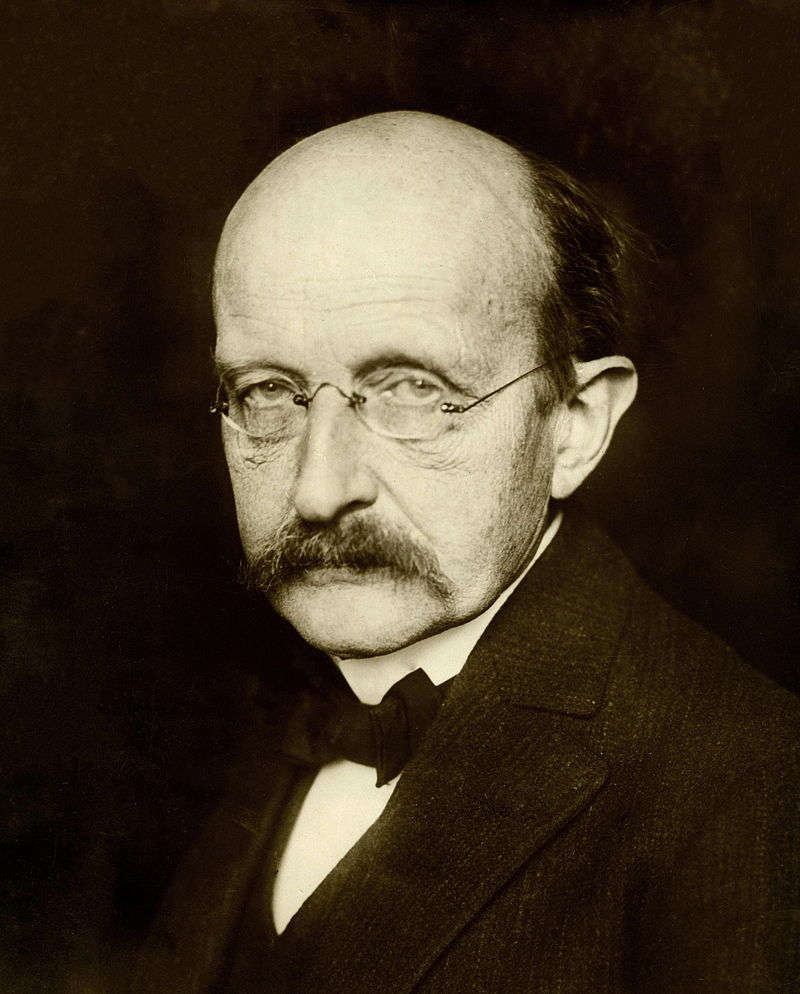
\includegraphics[width=3cm]{files/planck.jpg}}
	%
	\stopchronology
\end{frame}
%
\begin{frame}[planck01]
	\frametitle{La costante di Planck}
	\begin{block}{\only<1>{Il valore di $h$}\onslide<2->{Radiazione di corpo nero}}
		\begin{displaymath}
		    \only<1>{h = 6.626070 \cdot 10^{-34} J \cdot s}
			\onslide<2->{B_\nu = \frac{8 \pi h}{c^3} \nu^3 \frac{1}{e^{\frac{h \nu}{k T}}-1}}
		\end{displaymath}
	\end{block}
	\onslide<2->{Cos'� un corpo nero?}
	\begin{enumerate}
		\onslide<3->{\item Emettitore ideale: ad ogni frequenza, emette molta pi� energia di qualunque altro corpo alla stessa temperatura.}
		\onslide<4->{\item Emettitore diffuso: la radiazione � emessa isotropicamente}
	\end{enumerate}
\end{frame}
%
\subsection{Planck a scuola}
%
\begin{frame}[planck02]
	\frametitle{Misurare la costante di Planck}
	\begin{center}
		\begin{tikzpicture}[every node/.style={inner sep=0,outer sep=0}]
			\onslide<6->\node at (0,0) () {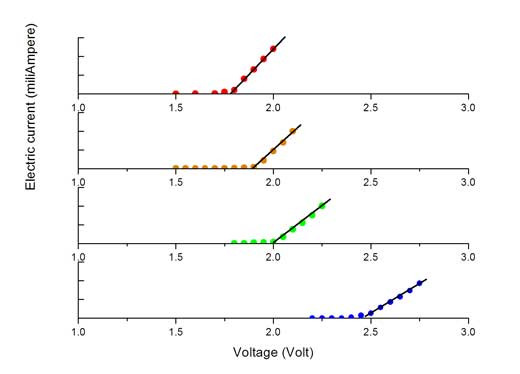
\includegraphics[width=5cm]{files/ledplot.jpg}};
			\onslide<1->\node at (4,0.5) () {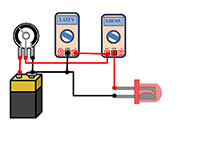
\includegraphics[width=3cm]{files/planckled.jpg}};
		\end{tikzpicture}	
	\end{center}
	\onslide<2-7>{\begin{block}{\onslide<2-6>{Materiali}\only<7>{Riferimenti}}
		\begin{itemize}
			\only<7>{\item \href{http://www.scienceinschool.org/2014/issue28/planck}{\textcolor{inaf}{Classroom fundamentals: measuring the Planck constant}}}
			\onslide<2-6>{\item 4 LED di 4 colori differenti (rosso, arancione, verde, blu)}
			\onslide<3-6>{\item una batteria}
			\onslide<4-6>{\item un tester (da utilizzare una volta come voltmetro e un'altra come amperometro)}
			\onslide<5-6>{\item un potenziometro da $1 k\Omega$}
		\end{itemize}
	\end{block}}
\end{frame}
%
\begin{frame}[corponero01]
	\frametitle{Visualizzare il corpo nero}
	\begin{center}
		\begin{tikzpicture}[every node/.style={inner sep=0,outer sep=0}]
			\onslide<1>\node at (0,0) () {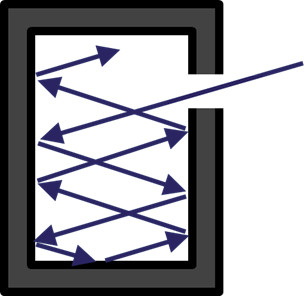
\includegraphics[width=2cm]{files/black_body.jpg}};
			\onslide<2->\node at (0,0) () {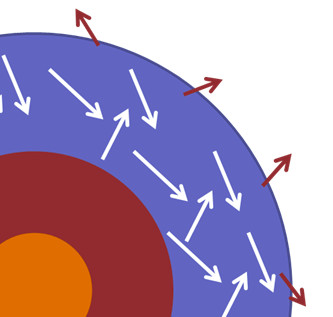
\includegraphics[width=2cm]{files/photosphere.jpg}};
		\end{tikzpicture}
	\end{center}
		\onslide<3->{\begin{block}{L'influenza di $h$ nell'universo}
			\only<3>{Se $h$ fosse dieci volte pi� piccola, delle semplici braci emetterebbero luce 1000 pi� intensa e a frequenze ultraviolette}
			\only<4>{Se $h$ fosse dieci volte pi� piccola, l'idrogeno non sarebbe pi� in grado di fondere in deuterio e produrre l'elio}
		\end{block}}
\end{frame}
%
\begin{frame}[corponero02]
	\frametitle{Il corpo nero a scuola}
	\begin{center}
		\only<1>{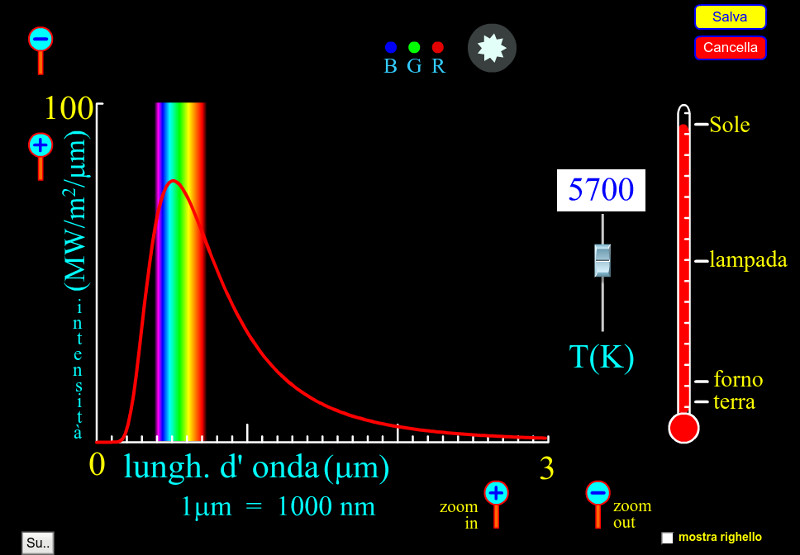
\includegraphics[width=8cm]{files/corponero.jpg}}
		\only<2>{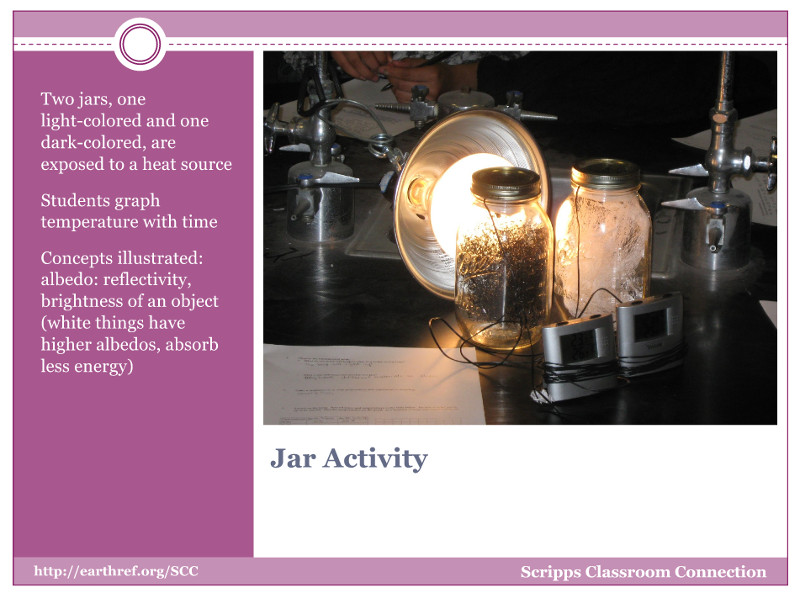
\includegraphics[width=8cm]{files/jaract.jpg}}
	\end{center}
	\begin{itemize}
		\only<1>{\item \href{https://phet.colorado.edu/en/simulation/blackbody-spectrum}{\textcolor{inaf}{Blackbody spectrum - PhET Interactive Simulations}}}
		\only<2>{\item \href{https://earthref.org/SCC/lessons/2012/electromagneticradiation/}{\textcolor{inaf}{Electromagnetic Radiation in the Atmosphere: Reflection, Absorption, and Scattering}}}
	\end{itemize}
\end{frame}
%
% Einstein
%
\section{Il contributo di Einstein}
%
\begin{frame}[timeline02]
	\frametitle{Gli articoli di Einstein}
	%---------------------timeline----------------%
	\startchronology[align=left, startyear=1897,stopyear=1922, height=0pt, startdate=false, stopdate=false, dateselevation=0pt, arrow=false, box=true]
	%
	\chronograduation[event][dateselevation=0pt]{1}
	%---------------------periods----------------%
	\chronoperiode[textstyle=\raggedleft\colorbox{inaf!50}, color=gr, startdate=false, bottomdepth=0pt, topheight=8pt, textdepth=-25pt,dateselevation=16pt, stopdate=false]{1904}{1905}{$E = h \nu$}
	%
	\stopchronology
	\begin{itemize}
		\item Equazione di Planck-Einstein
	\end{itemize}
\end{frame}
%
\begin{frame}[timeline03]
	\frametitle{Gli articoli di Einstein}
	%---------------------timeline----------------%
	\startchronology[align=left, startyear=1897,stopyear=1922, height=0pt, startdate=false, stopdate=false, dateselevation=0pt, arrow=false, box=true]
	%
	\chronograduation[event][dateselevation=0pt]{1}
	%---------------------periods----------------%
	\chronoperiode[textstyle=\raggedleft\colorbox{gr!50}, color=gr, startdate=false, bottomdepth=0pt, topheight=8pt, textdepth=-25pt,dateselevation=16pt, stopdate=false]{1904}{1905}{$E = h \nu$}
	\chronoperiode[textstyle=\raggedleft\colorbox{inaf!50}, color=gr, startdate=false, bottomdepth=0pt, topheight=8pt, textdepth=-25pt,dateselevation=16pt, stopdate=false]{1905}{1906}{$0, h\nu, 2h\nu, \cdots$}
	%
	\stopchronology
	\begin{itemize}
		\item Marzo 1906: quantizzazione energia oscillatore materiale
		\item Novembre 1906: la quantizzazione dell'energia degli oscillatori materiali spiega alcuni calori specifici
	\end{itemize}
\end{frame}
%
\begin{frame}[timeline04]
	\frametitle{Gli articoli di Einstein}
	%---------------------timeline----------------%
	\startchronology[align=left, startyear=1897,stopyear=1922, height=0pt, startdate=false, stopdate=false, dateselevation=0pt, arrow=false, box=true]
	%
	\chronograduation[event][dateselevation=0pt]{1}
	%---------------------periods----------------%
	\chronoperiode[textstyle=\raggedleft\colorbox{gr!50}, color=gr, startdate=false, bottomdepth=0pt, topheight=8pt, textdepth=-25pt,dateselevation=16pt, stopdate=false]{1904}{1905}{$E = h \nu$}
	\chronoperiode[textstyle=\raggedleft\colorbox{inaf!50}, color=gr, startdate=false, bottomdepth=0pt, topheight=8pt, textdepth=-25pt,dateselevation=16pt, stopdate=false]{1905}{1906}{$0, h\nu, 2h\nu, \cdots$}
	\chronoperiode[textstyle=\raggedleft\colorbox{inaf!50}, color=gr, startdate=false, bottomdepth=0pt, topheight=8pt, textdepth=-25pt,dateselevation=16pt, stopdate=false]{1908}{1909}{Corpo nero}
	%
	\stopchronology
	\begin{itemize}
		\item Le fluttuazioni nella densit� di energia emessa da un corpo nero confermano la doppia natura della luce
	\end{itemize}
\end{frame}
%
\begin{frame}[timeline05]
	\frametitle{Gli articoli di Einstein}
	%---------------------timeline----------------%
	\startchronology[align=left, startyear=1897,stopyear=1922, height=0pt, startdate=false, stopdate=false, dateselevation=0pt, arrow=false, box=true]
	%
	\chronograduation[event][dateselevation=0pt]{1}
	%---------------------periods----------------%
	\chronoperiode[textstyle=\raggedleft\colorbox{gr!50}, color=gr, startdate=false, bottomdepth=0pt, topheight=8pt, textdepth=-25pt,dateselevation=16pt, stopdate=false]{1904}{1905}{$E = h \nu$}
	\chronoperiode[textstyle=\raggedleft\colorbox{inaf!50}, color=gr, startdate=false, bottomdepth=0pt, topheight=8pt, textdepth=-25pt,dateselevation=16pt, stopdate=false]{1905}{1906}{$0, h\nu, 2h\nu, \cdots$}
	\chronoperiode[textstyle=\raggedleft\colorbox{inaf!50}, color=gr, startdate=false, bottomdepth=0pt, topheight=8pt, textdepth=-25pt,dateselevation=16pt, stopdate=false]{1908}{1909}{Corpo nero}
	\chronoperiode[textstyle=\raggedleft\colorbox{inaf!50}, color=gr, startdate=false, bottomdepth=0pt, topheight=8pt, textdepth=-25pt,dateselevation=16pt, stopdate=false]{1915}{1916}{$E_m-E_n = h \nu_{mn}$, $p_{mn} = h \nu_{mn}/c$}
	%
	\stopchronology
	\begin{itemize}
		\item Effetto fotoelettrico
		\item Casualit�
	\end{itemize}
\end{frame}
%
\subsection{L'effetto fotoelettrico}
%
\begin{frame}[fotoelettrico]
	\frametitle{L'effetto fotoelettrico a scuola}
	\begin{tikzpicture}[every node/.style={inner sep=0,outer sep=0}]
		\node at (0,0) () {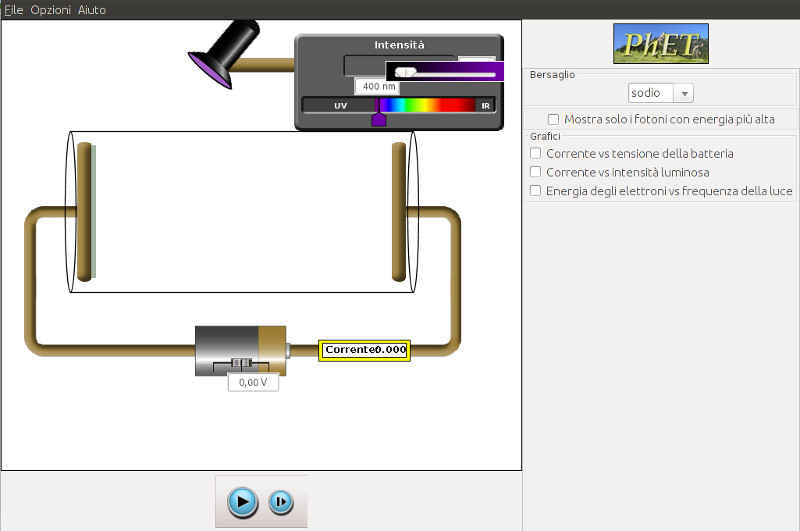
\includegraphics[width=5cm]{files/fotoelettrico.jpg}};
		\onslide<6>\node at (7,0.5) () {\href{http://iopscience.iop.org/article/10.1088/0031-9120/48/1/35/meta}{\textcolor{inaf}{Teaching the photoelectric}}};
		\onslide<6>\node at (7,0) () {\href{http://iopscience.iop.org/article/10.1088/0031-9120/48/1/35/meta}{\textcolor{inaf}{effect inductively}}};
	\end{tikzpicture}
	\begin{itemize}
		\item \href{https://phet.colorado.edu/en/simulation/photoelectric}{\textcolor{inaf}{Effetto fotoelettrico - PhET Interactive Simulations}}: applicazione Java
		\onslide<2->{\item Problem solving: }
		\onslide<3->{\item Stabilire le ipotesi/raccogliere informazioni}
		\onslide<4->{\item Analisi/controllo concettuale}
		\onslide<5->{\item Verifica e valutazione}
	\end{itemize}
\end{frame}
%
% La struttura dell'atomo
%
\section{La struttura dell'atomo}
%
\begin{frame}[timeline06]
	\frametitle{L'esperimento di Millikan}
	%---------------------timeline----------------%
	\startchronology[align=left, startyear=1915,stopyear=1940, height=0pt, startdate=false, stopdate=false, dateselevation=0pt, arrow=false, box=true]
	%
	\chronograduation[event][dateselevation=0pt]{1}
	%---------------------periods----------------%
	\chronoperiode[textstyle=\raggedleft\colorbox{inaf!50}, color=gr, startdate=false, bottomdepth=0pt, topheight=8pt, textdepth=-25pt,dateselevation=16pt, stopdate=false]{1916}{1917}{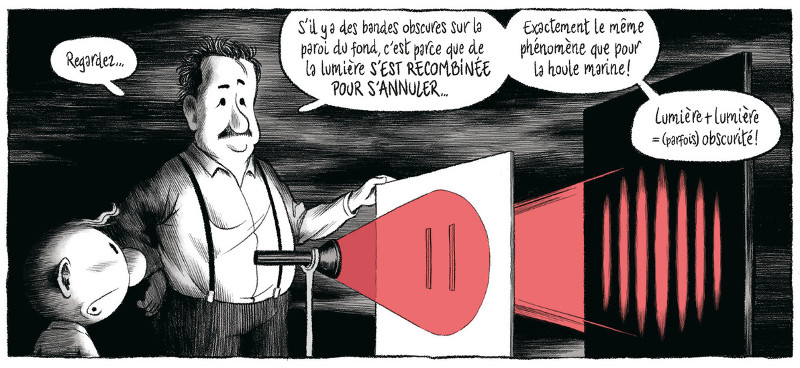
\includegraphics[width=4cm]{files/millikan.jpg}}
	%
	\stopchronology
\end{frame}
%
\begin{frame}[timeline06]
	\frametitle{L'esperimento di Compton}
	%---------------------timeline----------------%
	\startchronology[align=left, startyear=1915,stopyear=1940, height=0pt, startdate=false, stopdate=false, dateselevation=0pt, arrow=false, box=true]
	%
	\chronograduation[event][dateselevation=0pt]{1}
	%---------------------periods----------------%
	\chronoperiode[textstyle=\raggedleft\colorbox{inaf!50}, color=gr, startdate=false, bottomdepth=0pt, topheight=8pt, textdepth=-25pt,dateselevation=16pt, stopdate=false]{1916}{1917}{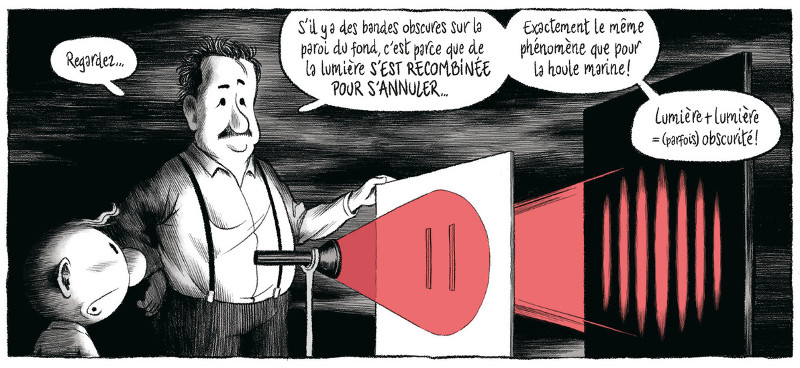
\includegraphics[width=4cm]{files/millikan.jpg}}
	\chronoperiode[textstyle=\raggedleft\colorbox{inaf!50}, color=gr, startdate=false, bottomdepth=0pt, topheight=8pt, textdepth=-25pt,dateselevation=16pt, stopdate=false]{1921}{1922}{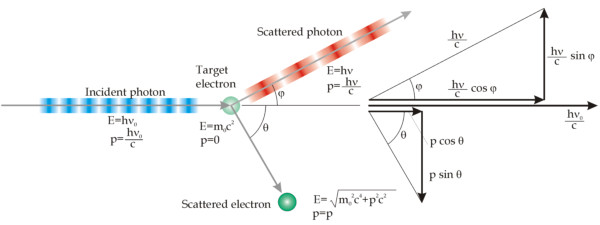
\includegraphics[width=6cm]{files/compton.jpg}}
	%
	\stopchronology
	\begin{itemize}
		\item $\lambda = \frac{h}{mc}$
	\end{itemize}
\end{frame}
%
\begin{frame}[timeline08]
	\frametitle{Onde di materia}
	%---------------------timeline----------------%
	\startchronology[align=left, startyear=1915,stopyear=1940, height=0pt, startdate=false, stopdate=false, dateselevation=0pt, arrow=false, box=true]
	%
	\chronograduation[event][dateselevation=0pt]{1}
	%---------------------periods----------------%
	\chronoperiode[textstyle=\raggedleft\colorbox{gr!50}, color=gr, startdate=false, bottomdepth=0pt, topheight=8pt, textdepth=-25pt,dateselevation=16pt, stopdate=false]{1916}{1917}{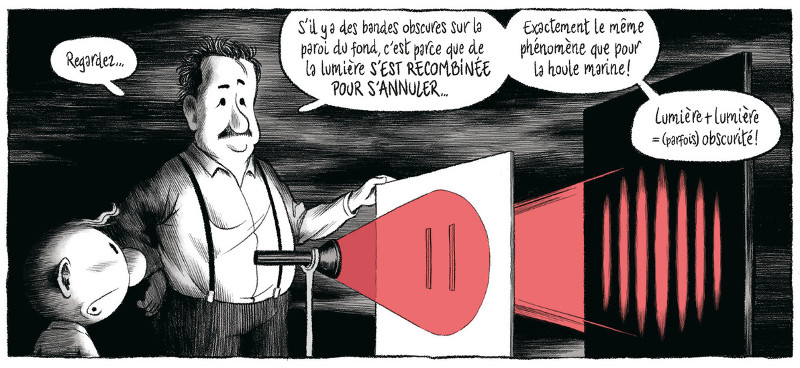
\includegraphics[width=4cm]{files/millikan.jpg}}
	\chronoperiode[textstyle=\raggedleft\colorbox{gr!50}, color=gr, startdate=false, bottomdepth=0pt, topheight=8pt, textdepth=-25pt,dateselevation=16pt, stopdate=false]{1921}{1922}{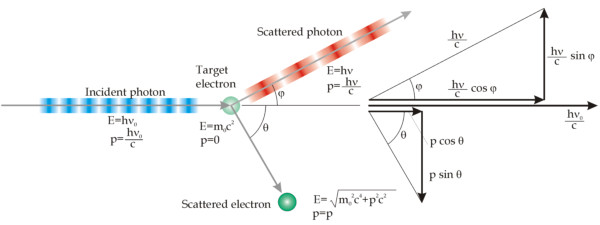
\includegraphics[width=6cm]{files/compton.jpg}}
	\chronoperiode[textstyle=\raggedleft\colorbox{inaf!50}, color=gr, startdate=false, bottomdepth=0pt, topheight=8pt, textdepth=-25pt,dateselevation=16pt, stopdate=false]{1924}{1925}{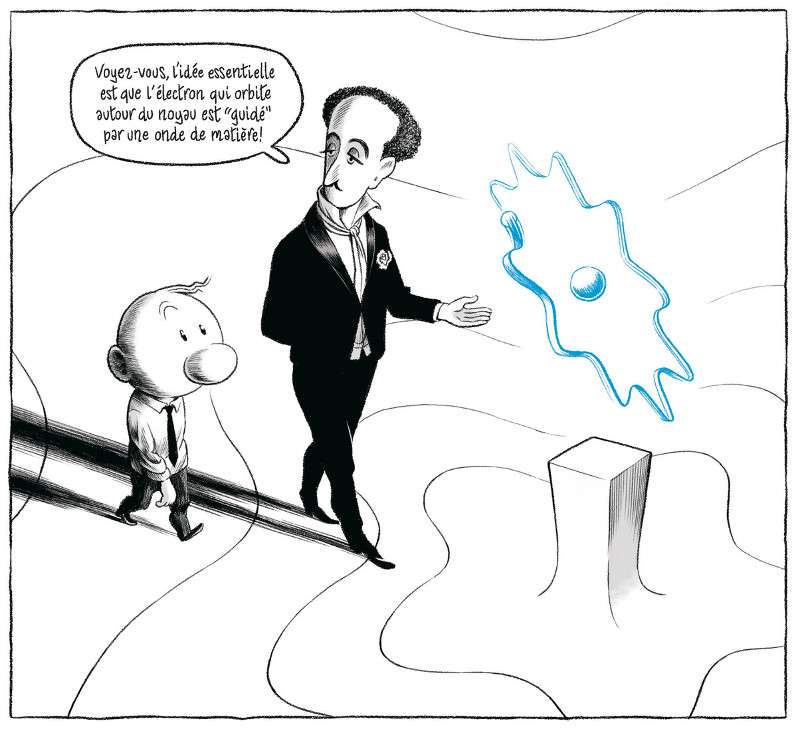
\includegraphics[width=4cm]{files/debroglie.jpg}}
	%
	\stopchronology
	\begin{itemize}
		\item Articoli indipendenti di Einstein e de Broglie
		\item $\nu = \frac{E}{c}, \; \lambda = \frac{h}{p}$
	\end{itemize}
\end{frame}
%
\begin{frame}[timeline09]
	\frametitle{Onde di materia}
	%---------------------timeline----------------%
	\startchronology[align=left, startyear=1915,stopyear=1940, height=0pt, startdate=false, stopdate=false, dateselevation=0pt, arrow=false, box=true]
	%
	\chronograduation[event][dateselevation=0pt]{1}
	%---------------------periods----------------%
	\chronoperiode[textstyle=\raggedleft\colorbox{gr!50}, color=gr, startdate=false, bottomdepth=0pt, topheight=8pt, textdepth=-25pt,dateselevation=16pt, stopdate=false]{1916}{1917}{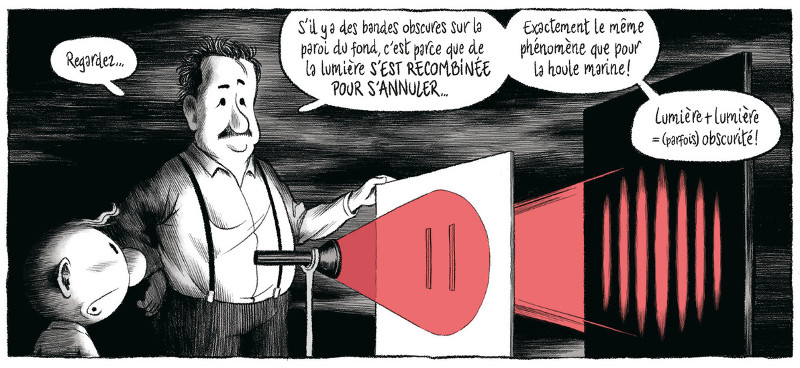
\includegraphics[width=4cm]{files/millikan.jpg}}
	\chronoperiode[textstyle=\raggedleft\colorbox{gr!50}, color=gr, startdate=false, bottomdepth=0pt, topheight=8pt, textdepth=-25pt,dateselevation=16pt, stopdate=false]{1921}{1922}{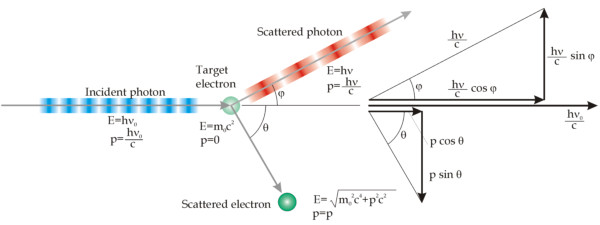
\includegraphics[width=6cm]{files/compton.jpg}}
	\chronoperiode[textstyle=\raggedleft\colorbox{gr!50}, color=gr, startdate=false, bottomdepth=0pt, topheight=8pt, textdepth=-25pt,dateselevation=16pt, stopdate=false]{1924}{1925}{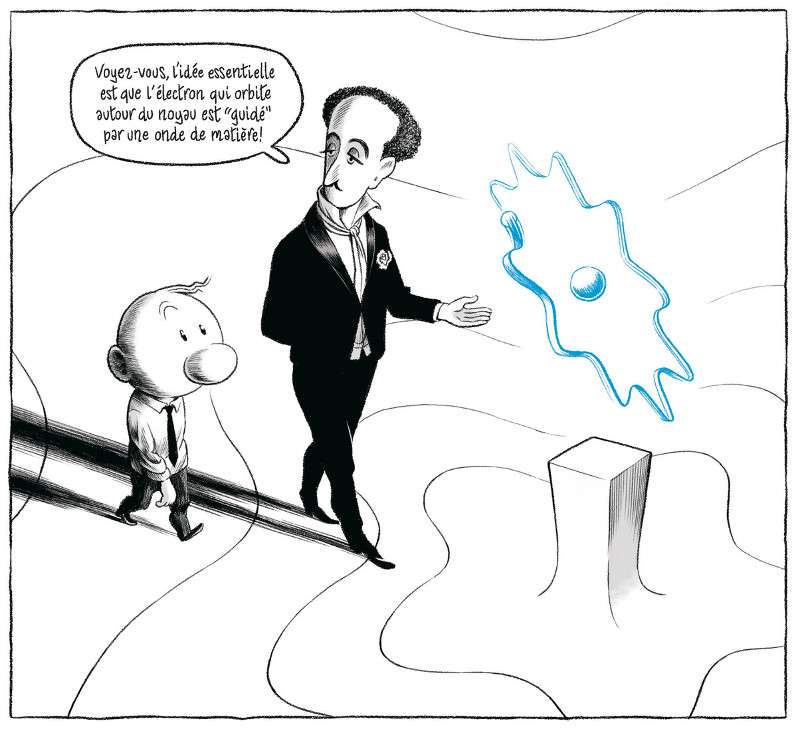
\includegraphics[width=4cm]{files/debroglie.jpg}}
	\chronoperiode[textstyle=\raggedleft\colorbox{inaf!50}, color=gr, startdate=false, bottomdepth=0pt, topheight=8pt, textdepth=-25pt,dateselevation=16pt, stopdate=false]{1925}{1926}{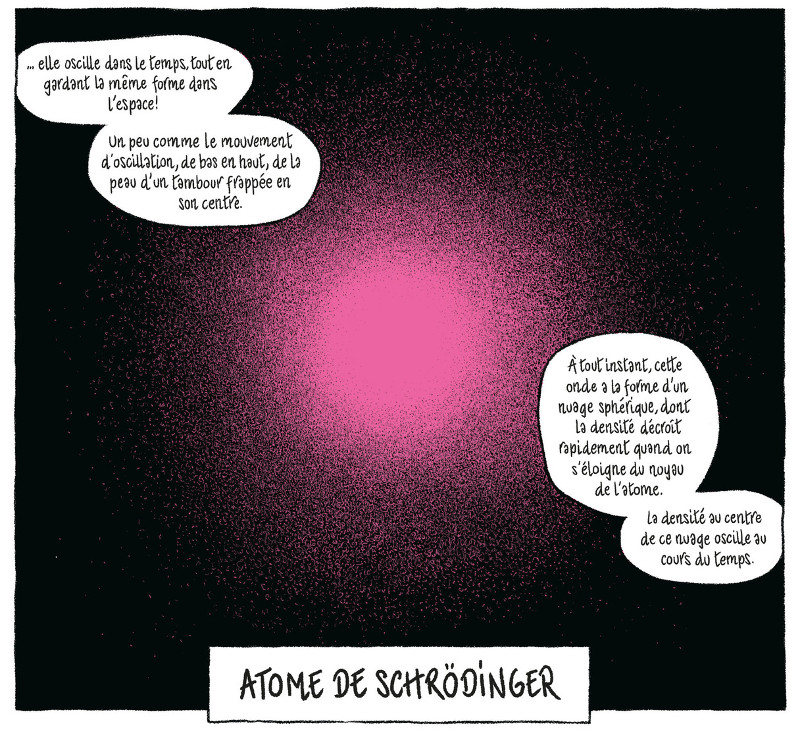
\includegraphics[width=4cm]{files/schroedinger.jpg}}
	%
	\stopchronology
	\begin{itemize}
		\item Equazione di Schroedinger
	\end{itemize}
\end{frame}
%
\begin{frame}[timeline09]
	\frametitle{Onde di materia}
	%---------------------timeline----------------%
	\startchronology[align=left, startyear=1915,stopyear=1940, height=0pt, startdate=false, stopdate=false, dateselevation=0pt, arrow=false, box=true]
	%
	\chronograduation[event][dateselevation=0pt]{1}
	%---------------------periods----------------%
	\chronoperiode[textstyle=\raggedleft\colorbox{gr!50}, color=gr, startdate=false, bottomdepth=0pt, topheight=8pt, textdepth=-25pt,dateselevation=16pt, stopdate=false]{1916}{1917}{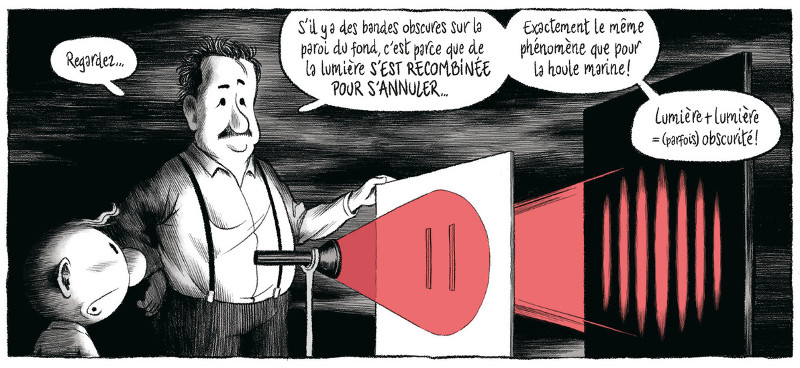
\includegraphics[width=4cm]{files/millikan.jpg}}
	\chronoperiode[textstyle=\raggedleft\colorbox{gr!50}, color=gr, startdate=false, bottomdepth=0pt, topheight=8pt, textdepth=-25pt,dateselevation=16pt, stopdate=false]{1921}{1922}{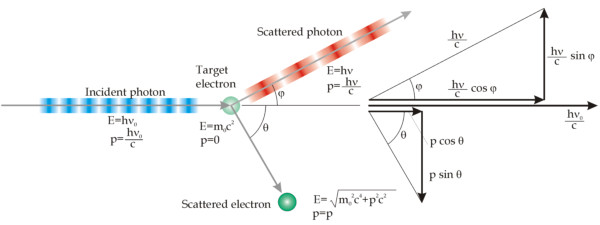
\includegraphics[width=6cm]{files/compton.jpg}}
	\chronoperiode[textstyle=\raggedleft\colorbox{gr!50}, color=gr, startdate=false, bottomdepth=0pt, topheight=8pt, textdepth=-25pt,dateselevation=16pt, stopdate=false]{1924}{1925}{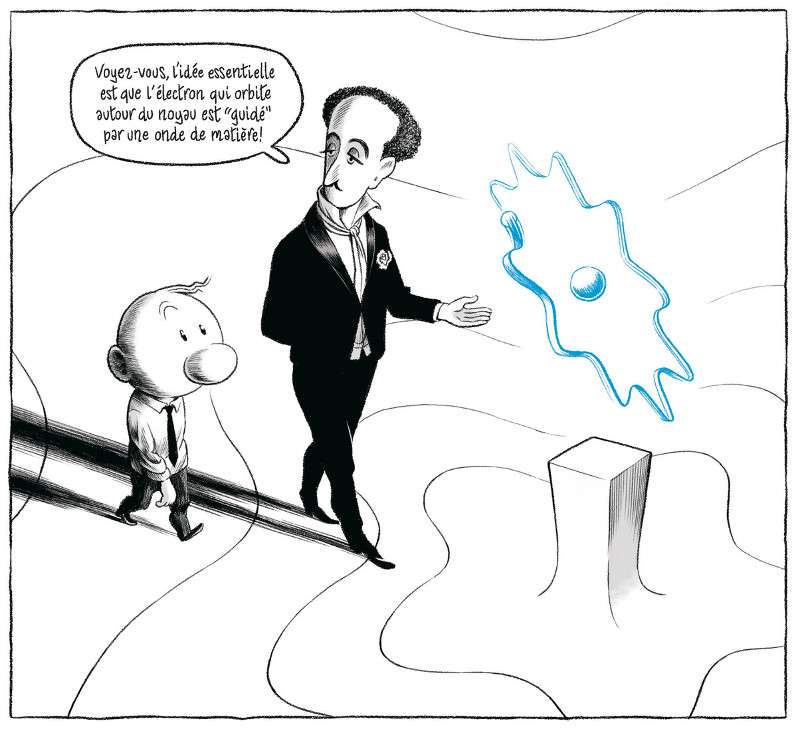
\includegraphics[width=4cm]{files/debroglie.jpg}}
	\chronoperiode[textstyle=\raggedleft\colorbox{gr!50}, color=gr, startdate=false, bottomdepth=0pt, topheight=8pt, textdepth=-25pt,dateselevation=16pt, stopdate=false]{1925}{1926}{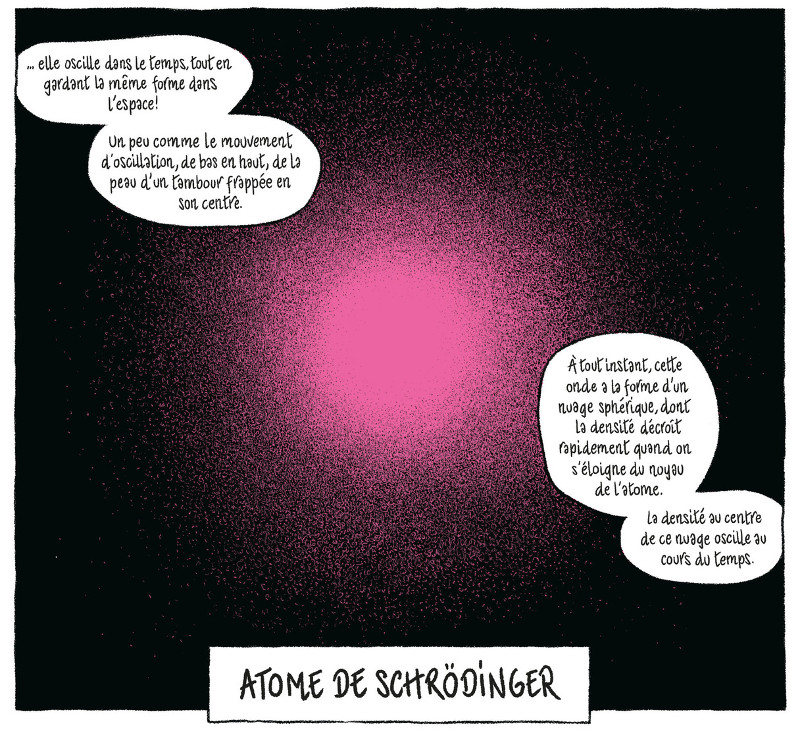
\includegraphics[width=4cm]{files/schroedinger.jpg}}
	\chronoperiode[textstyle=\raggedleft\colorbox{inaf!50}, color=gr, startdate=false, bottomdepth=0pt, topheight=8pt, textdepth=-25pt,dateselevation=16pt, stopdate=false]{1927}{1928}{Esperimento di Davisson e Germer}
	%
	\stopchronology
	\begin{itemize}
		\item Un fascio di elettroni attraversa un cristallo di nichel
	\end{itemize}
\end{frame}
%
\subsection{L'atomo di idrogeno}
%
\begin{frame}[idrogeno]
	\frametitle{Modelli \onslide<4->{e osservazione}}
	\begin{tikzpicture}[every node/.style={inner sep=0,outer sep=0}]
	\node at (0,0) () {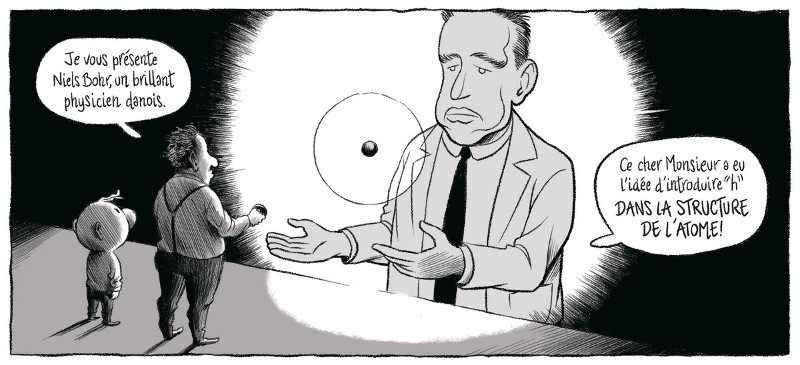
\includegraphics[width=5cm]{files/bohr.jpg}};
	\onslide<2->\node at (1,0.5) () {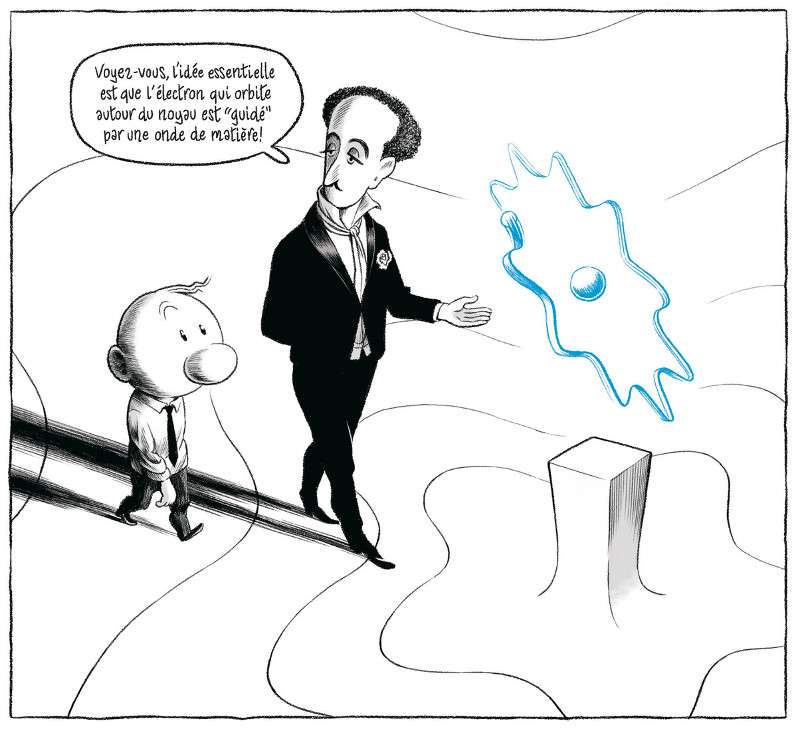
\includegraphics[width=5cm]{files/debroglie.jpg}};
	\onslide<3->\node at (2,1) () {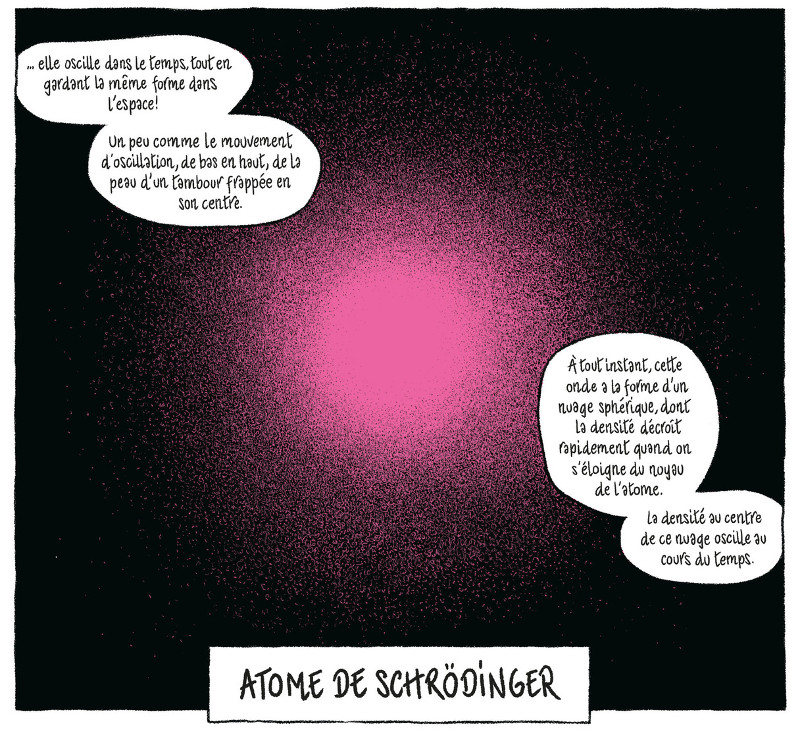
\includegraphics[width=5cm]{files/schroedinger.jpg}};
	\onslide<4->\node at (3,1.5) () {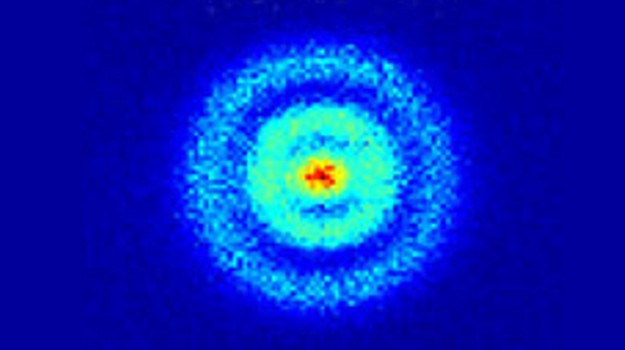
\includegraphics[width=5cm]{files/idrogeno.jpg}};
	\onslide<5->\node at (4,1.5) () {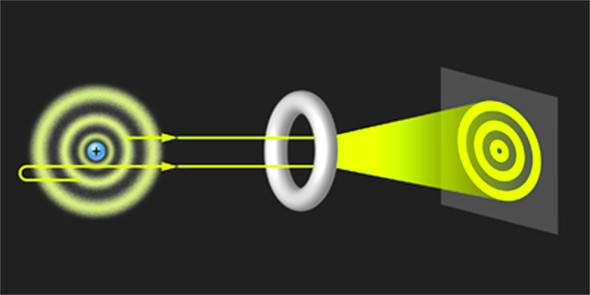
\includegraphics[width=5cm]{files/idrogeno_esperimento.jpg}};
	\end{tikzpicture}
	\begin{itemize}
		\onslide<4->{\item 2013}
	\end{itemize}
\end{frame}
%
\begin{frame}[risorse]
	\frametitle{Risorse didattiche}
	\begin{itemize}
		\onslide<1->{\item \href{http://scienzapertutti.infn.it/3-esperimenti-delle-due-fenditure-per-fotoni-ed-elettroni}{\textcolor{inaf}{Esperimento della doppia fenditura - Scienza per tutti}}}
		\onslide<2->{
			\begin{itemize}
				\item \href{https://www.tes.com/teaching-resource/young-s-double-slit-experiment-introduction-worksheet-for-6th-form-as-physics-11474274}{\textcolor{inaf}{Young's double slit experiment introduction worksheet for 6th form AS Physics}}
				\onslide<3->{\item \href{https://www.tes.com/teaching-resource/the-original-double-slit-experiment-6328282}{\textcolor{inaf}{The Original Double Slit Experiment}}}
			\end{itemize}}
		\onslide<4>{\item \href{http://astroedu.iau.org/it/activities/1502/rompiamo-le-particelle/}{\textcolor{inaf}{Rompiamo le particelle - astroEDU}}}
	\end{itemize}
\end{frame}
%
\section{Bibliografia}
%
\begin{frame}[bibliografia]
	\frametitle{Bibliografia}
	\begin{center}
		{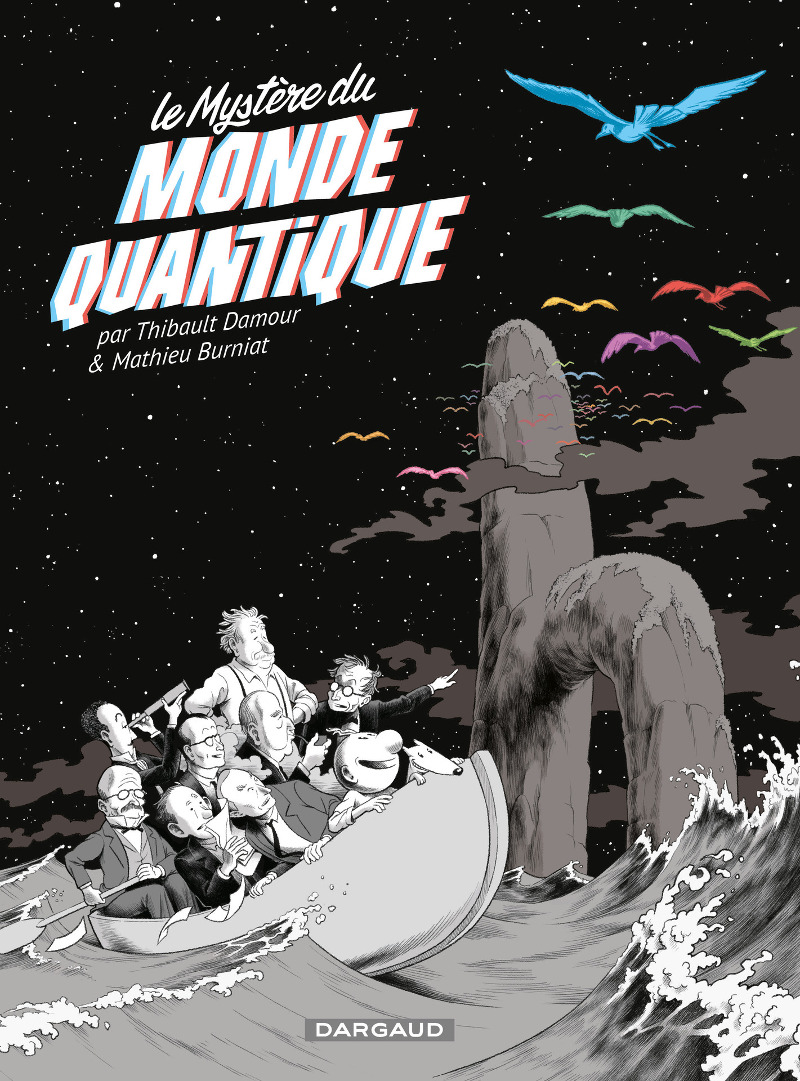
\includegraphics[width=5cm]{files/mondo_quantistico.jpg}}
	\end{center}
\end{frame}
\end{document}
